%!TEX root = ../thesis.tex
%*******************************************************************************
%*********************************** First Chapter *****************************
%*******************************************************************************

\chapter{PENDAHULUAN}  %Title of the First Chapter

\ifpdf
    \graphicspath{{Chapter1/Figs/Raster/}{Chapter1/Figs/PDF/}{Chapter1/Figs/}}
\else
    \graphicspath{{Chapter1/Figs/Vector/}{Chapter1/Figs/}}
\fi


%********************************** %First Section  **************************************
\section{Latar Belakang} %Section - 1.1 


Indonesia sangat rawan terhadap musibah bencana alam baik yang terjadi dalam skala kecil (daerah) maupun besar (nasional). Jumlah korban, kerugian harta benda, kerusakan prasarana dan sarana, cakupan luas wilayah yang terkena bencana dan dampak sosial ekonomi yang ditimbulkan menjadi parameter penggolongan skala tersebut (UU No.24/2007 Pasal 7(2)). 

Indonesia memiliki banyak sekali catatan bencana alam dengan skala besar. Seperti gempa bumi 9.3 skala Ritcher dan tsunami besar yang telah menewaskan sebanyak 230.000 jiwa di Aceh dan 14 negara lain tahun 2004. Juga sebuah gempa tektonik di Yogyakarta dengan kekuatan 6.2 skala Ritcher yang memakan korban sebesar 6.234 jiwa tahun 2006.

Di Indonesia, banjir merupakan bencana alam yang paling sering terjadi, disusul dengan tanah longsor, angin puyuh dan gempa bumi. Hal tersebut dapat dilihat pada data tentang banyaknya desa terdampak menurut jenis bencana alam dalam rentang waktu 2011-2014 oleh Badan Pusat Statistik (BPS) yang disajikan dalam Gambar~\ref{fig:chart_desa_terdampak}.

\begin{figure}[ht]
\centering
 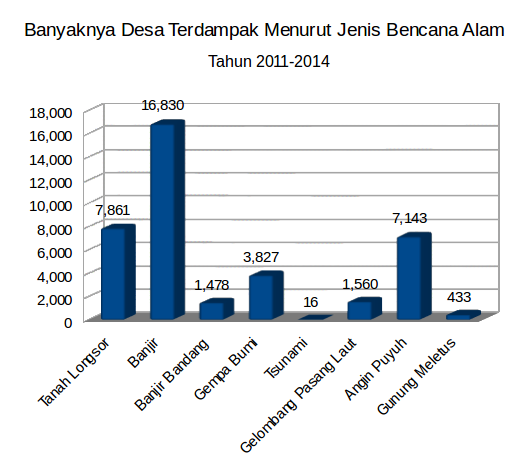
\includegraphics[width=0.8\textwidth]{chart_desa_terdampak}
 \caption{Data Bencana Alam di Indonesia 2011-2014}
 \captionsetup{font={footnotesize}}
 \caption*{Sumber: http://bps.go.id/index.php/linkTabelStatis/1764 (diakses tanggal 19 Juni 2016)}
 \label{fig:chart_desa_terdampak}   
\end{figure}

Prioritas utama ketika terjadi bencana alam adalah meminimalisir jatuhnya korban dengan cara penyelamatan pasca bencana. Salah satu badan yang mengurus tentang pencarian dan penyelamatan korban bencana alam adalah Badan SAR Nasional (BASARNAS). BASARNAS diketahui memiliki kemampuan personel yang cukup mumpuni, namun memiliki keterbatasan pada jumlah personel dan perlengkapan yang ada. Hal tersebut membuat melambatnya proses pencarian dan evakuasi korban yang mengakibatkan semakin bertambahnya jumlah korban jiwa.

Penelitian tentang robot yang dirancang untuk membantu manusia mengevakuasi korban bencana alam sebelumnya telah dilakukan. Murphy (2014) dalam bukunya menyebut robot-robot tersebut dengan nama rescue robot. pada jenis UGV, pergerakan relatif terbatas membuat kecepatannya untuk mencari korban dalam area yang besar menjadi lambat. Penelitian pada jenis UAV biasanya hanya terbatas pada pengkondisian bencana alam yang terlihat jelas perbedaannya dengan latar belakang yang sederhana.

Untuk meningkatkan proses pencarian korban, digagaslah sebuah sistem pencarian korban bencana alam menggunakan penginderaan dari udara secara otomatis yang diberi nama Aerial Search and Traverse Robot (AESTRO). Sistem akan menggunakan sebuah Unmanned Aerial Vehicle (UAV) yang terpasang dengan kamera lalu dijalankan di atas area bencana. Berbeda dari penggunaan UAV pada umumnya yang harus dimonitor secara langsung oleh manusia, AESTRO diharapkan mampu secara otomatis mendeteksi lokasi korban bencana alam beserta banyaknya korban yang terdeteksi dalam suatu area.

\begin{figure}[ht]
  \centering
  \begin{subfigure}[b]{0.49\textwidth}
    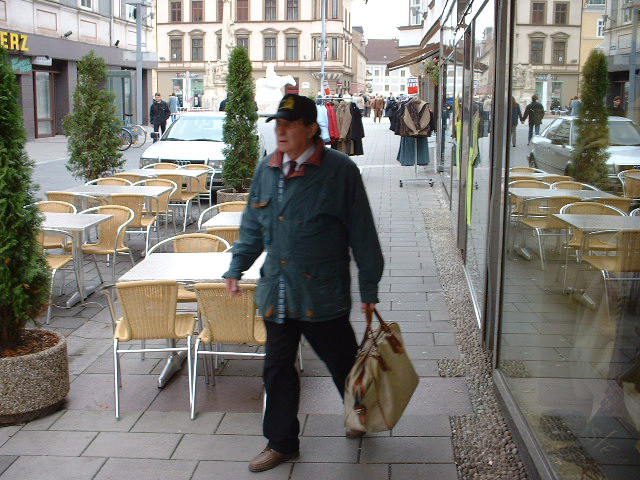
\includegraphics[width=\textwidth]{pedestrian}
    \caption{}
  \end{subfigure}             
  \begin{subfigure}[b]{0.49\textwidth}
    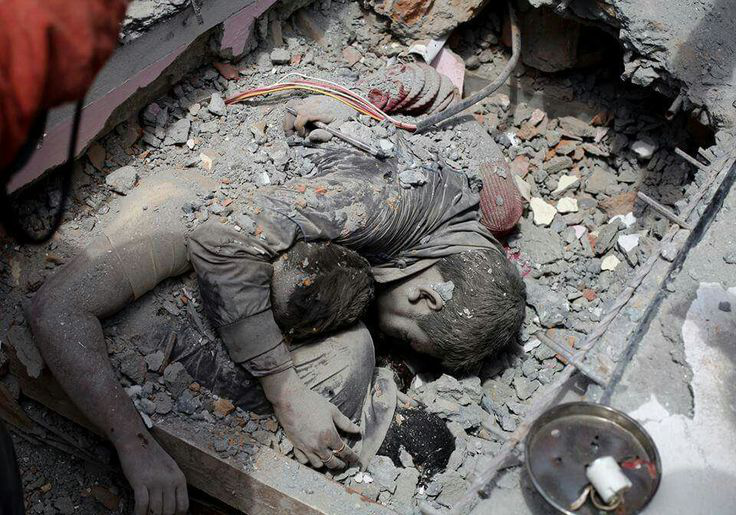
\includegraphics[width=\textwidth]{victim}
    \caption{}
  \end{subfigure}
  \caption{Perbedaan Citra (a) Pejalan Kaki (b) Korban Gempa Bumi}
  \captionsetup{font={footnotesize}}
  \caption*{Sumber: (a) INRIA Dataset (b) http://www.nepalbritain.com/ (diakses tanggal 20 Juni 2016)}
  \label{fig:comp_pedestrian_victim}
\end{figure}

Penelitian tentang pencarian korban bencana alam merupakan subjek yang menarik dikarenakan korban bencana alam terkadang ditemukan dalam kondisi warna yang bercampur dengan keadaan sekitar. Hal tersebut dapat dilihat pada Gambar~\ref{fig:comp_pedestrian_victim} (a) dapat dibedakan secara jelas warna antara manusia dan latar belakang sedangkan pada gambar (b) warna dari korban bercampur dengan reruntuhan bangunan di sekitarnya.

%Perlu diperhatikan juga bahwa terdapat perbedaan yang sangat mencolok tentang bagaimana manusia dan komputer melihat sebuah citra. Terlihat dari Gambar1.3 bahwa komputer melihat sebuah citra berdasarkan data warna yang ada. Pada penelitian ini, data warna tersebut akan digunakan sebagai masukan pada Deep Learning dan diolah pada masing masing layer untuk akhirnya mendapatkan keluaran berupa keputusan bahwa citra yang didapatkan merupakan manusia atau bukan. 

Untuk melakukan proses Deep Learning, diperlukan juga sebuah gambar masukan yang sangat banyak untuk proses learning yang disebut dataset. Untuk saat ini, masih sulit ditemukan sebuah dataset khusus tentang korban bencana alam yang benar-benar mencerminkan kondisi bencana yang kacau. Penelitian ini juga diharapkan mampu membuat dan mempublikasikan dataset khusus tentang korban bencana alam.                                                  


%********************************** %Second Section  *************************************
\section{Tujuan Proyek Akhir} %Section - 1.2

Tujuan dari penelitian ini adalah merancang sistem pencarian korban bencana alam yang mampu mendeteksi korban secara akurat lalu menandai pada bagian mana korban paling banyak ditemukan. Selain itu, penelitian ini juga akan mempublikasikan dataset sebanyak 500 gambar korban bencana alam terdiri dari train dan test untuk penelitian selanjutnya.

%********************************** % Third Section  *************************************
\section{Rumusan Masalah}  %Section - 1.3 
\label{section1.3}

Dari penjelasan sebelumnya, permasalahan yang akan di bahas dalam penelitian ini yaitu:
\begin{enumerate}
 \item Bagaimana mendeteksi korban bencana alam dari gambar kondisi bencana alam menggunakan Deep Learning?
 \item Bagaimana menentukan lokasi paling banyak terdapat korban bencana alam dari gambar gambar yang diperoleh?
 \item Bagaimana membuat dataset korban bencana alam untuk riset selanjutnya?
\end{enumerate}

%********************************** % Forth Section  *************************************
\section{Batasan Masalah}  %Section - 1.4

Dari rumusan masalah tersebut, akan dilakukan batasan masalah yaitu:
\begin{enumerate}
 \item Dilakukan pada satu jenis kondisi dampak bencana alam.
 \item Pembahasan hanya mengenai proses pengolahan gambar.
 \item Uji coba dilakukan pada pencahayaan yang cukup pada pagi hingga sore hari.
 \item Korban bencana harus terlihat utuh atau terlihat sebagian tubuh yang atas.
\end{enumerate}

%********************************** % Fifth Section  *************************************
\section{Metodologi Proyek Akhir}  %Section - 1.5 
Metodologi yang digunakan pada penelitian tugas akhir ini adalah sebagai berikut:
\begin{enumerate}
 \item Studi Literatur
 \begin{itemize}
    \item Mencari dan mempelajari struktur medan bencana yang tidak beraturan serta mempelajari model pencarian korban pada saat bencana yang dilakukan oleh robot USAR
    \item Mencari dan mempelajari simulator webots untuk mensimulasikan model pergerakan pada robot.
    \item Mencari dan mempelajari pustaka mengenai desain mekanika mobile robot SAR, baik yang menggunakan system gerak beroda maupun berkaki.
 \end{itemize}
 \item Desain Meknika Robot iSRo
 \begin{itemize}
    \item Membuat desain mekanika Robot iSRo dengan menggunakan software simulasi Webots.
    \item Melakukan pengujian terhadap kualitas, stabilitas serta model-model pergerakan yang diperkirakan dapat dijalankan pada Robot iSRo.
 \end{itemize}
 \item Proses pembuatan mekanika Robot iSRo serta program simulasi Webots dan komunikasi serial interface
 \item Implementasi program 
 Berdasarkan perencanaan yang telah ditentukan sebelumnya dibuat model meknisme Robot iSRo pada simulator untuk dilakukan simulasi manual lalu dibuat program untuk simulasi autonomosnya setelah itu baru program diimplementasikan pada Robot iSRo yang sesungguhnya (real Robot iSRo). Sedangkan untuk mengoperasikannya Robot iSRo dilakukan pengendalian dari jarak jauh dengan media komunikasi wireless.
 \item Pengujian dan Analisa Data.
 \begin{itemize}
    \item Membahas mengenai pengujian desain dan model-model pergerakan, yang telah dilakukan di simulator Webots ketika diterapkan pada Robot iSRo yang sesungguhnya. 
    \item Melakukan analisa dari desain dan model pergerakan Robot iSRo yang telah dicapai pada saat pengujian
 \end{itemize}
\end{enumerate}
1. Studi literatur.


%********************************** % Sixth Section  *************************************
\section{Sistematika Penulisan}  %Section - 1.6 

Sistematika penulisan berisi tentang bagaimana menyajikan laporan proyek akhir. Sistematika yang akan diuraikan dalam proposal proyek akhir ini terbagi dalam bab-bab yang akan dibahas sebagai berikut:
\\
\\
BAB 1 : PENDAHULUAN

Berisi latar belakang pembuatan proyek akhir, rumusan masalah dalam proyek akhir ini, batasan masalah, tujuan dari rumusan masalah, luaran yang diharapkan, metedologi untuk menyelesaikan proyek akhir ini, dan sistematika penulisan.
\\
\\
BAB II : STUDI PUSTAKA

Berisi tentang tinjauan pustaka penelitian sebelumnya dan teori penunjang yang mendukung dalam perencanaan serta pembuatan proyek akhir ini. Teori yang ditinjau mengacu pada penelitian-penelitian sebelumnya tentang macam-macam penelitian tentang \textit{disaster robot}, penelitian \textit{Deep Learning}, dan penggunaan \textit{Deep Learning Framework}.
\\
\\
BAB III : PERANCANGAN DAN PEMBUATAN SISTEM

Berisi tentang gambaran umum sistem yang akan dibangun, desain perancangan komputer, hardware dan komunikasi yang digunakan, serta arsitektur Deep Learning yang akan digunakan.
\\
\\
BAB IV : PENGUJIAN DAN ANALISA SISTEM

Berisi tentang pengujian dari masing-masing bagian sistem dan pengujian sistem sementara. Pada bab ini akan diperlihatkan hasil yang telah diterapkan dan pada bagian mana dapat dilakukan penyempurnaan.
\\
\\
BAB V : PENUTUP

Berisi kesimpulan dan analisa sistem dari proyek akhir yang telah didapat serta saran-saran untuk pengembangan selanjutnya.

% \nomenclature[z-DEM]{DEM}{Discrete Element Method}
% \nomenclature[z-FEM]{FEM}{Finite Element Method}
% \nomenclature[z-PFEM]{PFEM}{Particle Finite Element Method}
% \nomenclature[z-FVM]{FVM}{Finite Volume Method}
% \nomenclature[z-BEM]{BEM}{Boundary Element Method}
% \nomenclature[z-MPM]{MPM}{Material Point Method}
% \nomenclature[z-LBM]{LBM}{Lattice Boltzmann Method}
% \nomenclature[z-MRT]{MRT}{Multi-Relaxation 
% Time}
% \nomenclature[z-RVE]{RVE}{Representative Elemental Volume}
% \nomenclature[z-GPU]{GPU}{Graphics Processing Unit}
% \nomenclature[z-SH]{SH}{Savage Hutter}
% \nomenclature[z-CFD]{CFD}{Computational Fluid Dynamics}
% \nomenclature[z-LES]{LES}{Large Eddy Simulation}
% \nomenclature[z-FLOP]{FLOP}{Floating Point Operations}
% \nomenclature[z-ALU]{ALU}{Arithmetic Logic Unit}
% \nomenclature[z-FPU]{FPU}{Floating Point Unit}
% \nomenclature[z-SM]{SM}{Streaming Multiprocessors}
% \nomenclature[z-PCI]{PCI}{Peripheral Component Interconnect}
% \nomenclature[z-CK]{CK}{Carman - Kozeny}
% \nomenclature[z-CD]{CD}{Contact Dynamics}
% \nomenclature[z-DNS]{DNS}{Direct Numerical Simulation}
% \nomenclature[z-EFG]{EFG}{Element-Free Galerkin}
% \nomenclature[z-PIC]{PIC}{Particle-in-cell}
% \nomenclature[z-USF]{USF}{Update Stress First}
% \nomenclature[z-USL]{USL}{Update Stress Last}
% \nomenclature[s-crit]{crit}{Critical state}
% \nomenclature[z-DKT]{DKT}{Draft Kiss Tumble}
% \nomenclature[z-PPC]{PPC}{Particles per cell}